\documentclass[tikz, border=1mm]{standalone}

%% FEYNMAN DIAGRAMS
\usepackage[compat=1.1.0]{tikz-feynman}
\tikzfeynmanset{warn luatex=false}
%% CMS COMMANDS (slightly modified since I could not fix some ifthenelse with booleans)
\usepackage{ptdr-definitions}
\usepackage{heppennames2}
% CUSTOM COMMANDS
\input{../lib/definitions}

\begin{document}
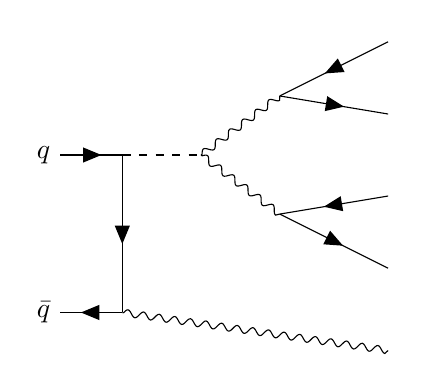
\begin{tikzpicture}
  \begin{feynman}
    \vertex (i1) at (0,2.5) {\(q\)};
    \vertex (i2) at (0,0.5) {\(\bar{q}\)};

    \vertex [right=1.0 of i1] (a);
    \vertex [right=1.0 of i2] (b);
    \vertex [right=1.0 of a]  (c);
    \vertex (d) at (3,3.25);
    \vertex [below=1.5 of d]  (e);

    \vertex (f5) at (4.5,0) {\(\PGg\)};
    \vertex [above=1.0 of f5] (f4) {\(\PAl\)};
    \vertex [above=1.0 of f4] (f3) {\(\Pl\)};
    \vertex [above=1.0 of f3] (f2) {\(\PAl\)};
    \vertex [above=1.0 of f2] (f1) {\(\Pl\)};

    \diagram* {
      (i1) -- [fermion] (a) -- [fermion] (b) -- [fermion] (i2),
      (a) -- [scalar, edge label=\(\PH\)] (c),
      (c) -- [boson, edge label=\(\PZ\)] (d),
      (c) -- [boson, edge label=\(\PZ\)] (e),
      (b) -- [boson] (f5),
      (f1) -- [fermion] (d) -- [fermion] (f2),
      (f3) -- [fermion] (e) -- [fermion] (f4),
    };
  \end{feynman}
\end{tikzpicture}
\end{document}

